\documentclass[10pt]{article}

\usepackage{verbatim}
\usepackage{amsmath}
\usepackage{enumerate}
\usepackage{url}
\usepackage{geometry}
\usepackage{amsthm}
\usepackage{graphicx}
\usepackage{hyperref}
\usepackage{subfigure}
%\usepackage[justification=centering]{caption}
%\linespread{2}

%Title information for the entirety of the class document
\title{Hoverboard Construction and Experimentation using ROS}
\author{Kevin Chiang, Tony Schneider, Lina Yu, Baoliang Zhao\\(Point Person: Tony Schneider)}
\date{Due 9/26/2013}
\begin{document}
\maketitle

\section*{Introduction}
A robot can be thought of as a series of simple components working in unison to produce seemingly complicated behavior.  However, this requires each component to work as a cohesive whole -- a task which is daunting (to say the least). \emph {ROS} (the \textbf{R}obot \textbf{O}perating \textbf{S}ystem), an open source framework for robotics programming, was created to facilitate the use and communication of an arbitrary amount of these components (called \emph{nodes}). 

Using ROS in conjunction with several pre-written ROS nodes used to control radio and serial communication provides a platform for learning the basics of robotics. A hovercraft was constructed using relatively simple materials (i.e., styrofoam, tape, and plastic), and powered via 6 GW-EDF40 thrusters and a battery.  ROS was used to control each individual thruster with an Xbox controller, as well as fire thrusters in combination with one another to provide for more complicated translational movements.  This experience provided first hand experience in the construction and design of a simple robot, as well as an understanding of the fine tuning and manual evaluation required when working with mechanical systems.

\section*{Hovercraft Construction and Design}
The base of the hovercraft base was made of styrofoam roughly 1.5" thick.  A circular base was chosen for the simplicity of obtaining a balanced weight distribution and skirt construction.   The diameter of the base was 16.5".  The size of the base was chosen primarily because it was the size of the available template.  However, the size seems like a good compromise between a light weight and a surface area large enough to fit all of the individual components.  

The skirt was constructed by first drawing a circle 0.75 inches larger than the base with a spacer on the plastic sheeting.  The sheeting was then cut down, and taped to the bottom of the hovercraft.  Lastly, a circle 1.5 inches smaller than the base was drawn on the bottom sheet and cut out of the inner circle to create the skirt.  The first attempt resulted in a skirt that was too small due to a problem with taping the sheet to the base evenly, but the second attempt was a success.  

\begin{figure}
\centering
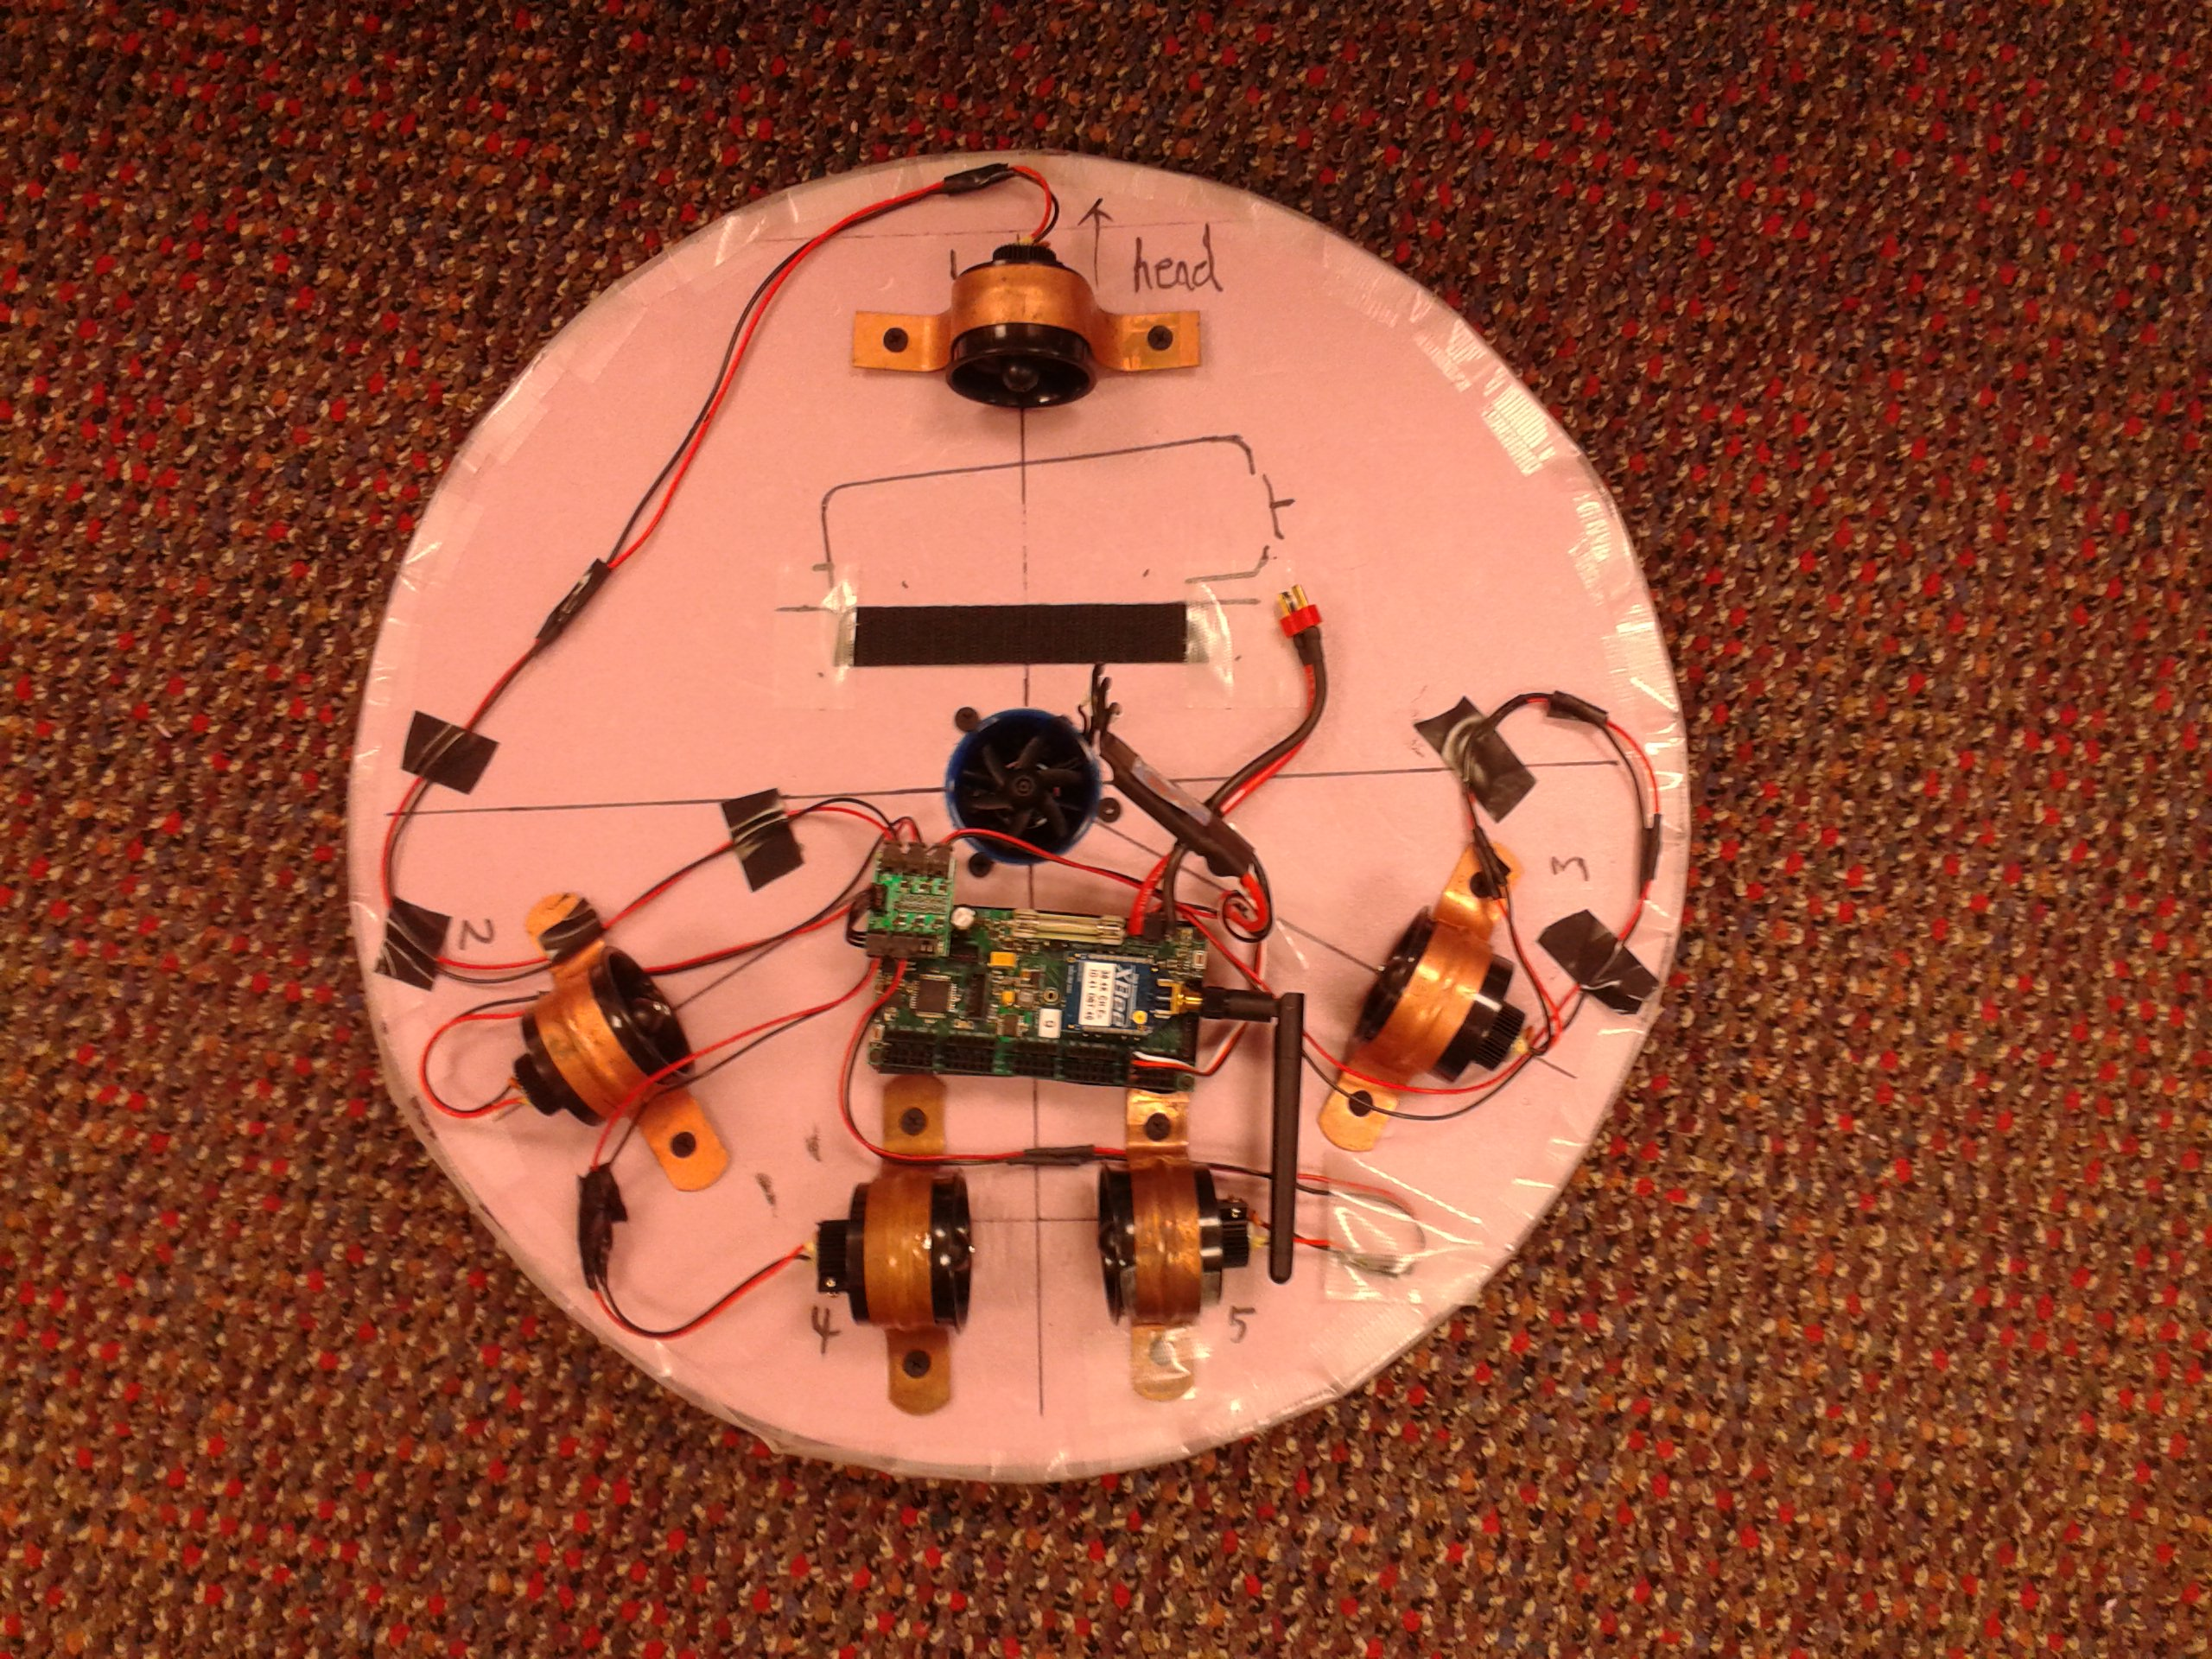
\includegraphics[width=.75\textwidth]{images/hovercraft}
\caption{Overhead view of the hovercraft after construction was completed}
\label{hovercraft}
\end{figure}

The configuration of the thrusters was adopted from the instructor's design.  The three translational thrusters were separated by 120� separation each around the circumference of the hovercraft (thrusters 1, 2, and 3 in figure~\ref{hovercraft}), and the two rotational thrusters are set in direct opposition to one another at the base of the craft (thrusters 4 and 5 in figure~\ref{hovercraft}). This design was adopted primarily for its relatively straightforward way of implementing left and right translation using two thrusters simultaneously (with a small amount of trigonometry), as well as the simplicity of rotation (i.e., by firing a single rotational thruster).  


This design required thrusters 1 and 3 to be relatively far away from the thrust controller on the hovercraft, so it was necessary to solder an extension to these thrusters.  However, thrusters 2, 4, and 5 were close enough to the controller that they could be attached without modifications.  The wires themselves were left unlabeled, but the thrusters corresponding to each input on the thrust controller were labeled with their corresponding connector number (as seen in figure~\ref{hovercraft}).

The positioning of the thrusters and board shifted the center of gravity of the hovercraft considerably.  To ameliorate this shift, the hoverboard controller and battery were mounted on the two sides of the lift thruster (center of figure~\ref{hovercraft}), to shift the center of gravity back towards the center of the hovercraft.  

\section*{ROS Setup and Experiments}
ROS was installed using the ready-to-run virtual machine provided on \url{http://nootrix.com/wp-content/uploads/2013/01/rosGroovyGalapagos.ova}.  The VM includes all core libraries required to compile and run both C++ and Python ROS nodes, specifically the roscpp library which is a set of bindings used to link C++ code to ROS (located at /opt/ros/groovy/share/roscpp in the VM installation).   

ROS provides several amenities besides libraries to aid in the design, testing, and execution of a robot.  Among these is a launch file, which allows an arbitrary number of nodes to be launched together.  One of the provided launch files ("hovercraft.launch") initially deployed three nodes: rxtx, HoverboardLL, and HoverCraft.  The launch file also allows various parameters to be configured on each node; for example, the rxtx node needs the serial port used for radio communication.  This is set to /dev/ttyUSB0 by default, but can easily be altered in the launch file.

In addition to the three nodes that are deployed in the initial launch file, there are currently an additional two nodes being launched. The first, XboxTeleop, is used to control communications between the Xbox Controller and the thrusters.   The second, GyroLimiter, caps the power of the rotational thrusters to the maximum rotation rate detected by the hoverboard.  

\begin{figure}
\centering
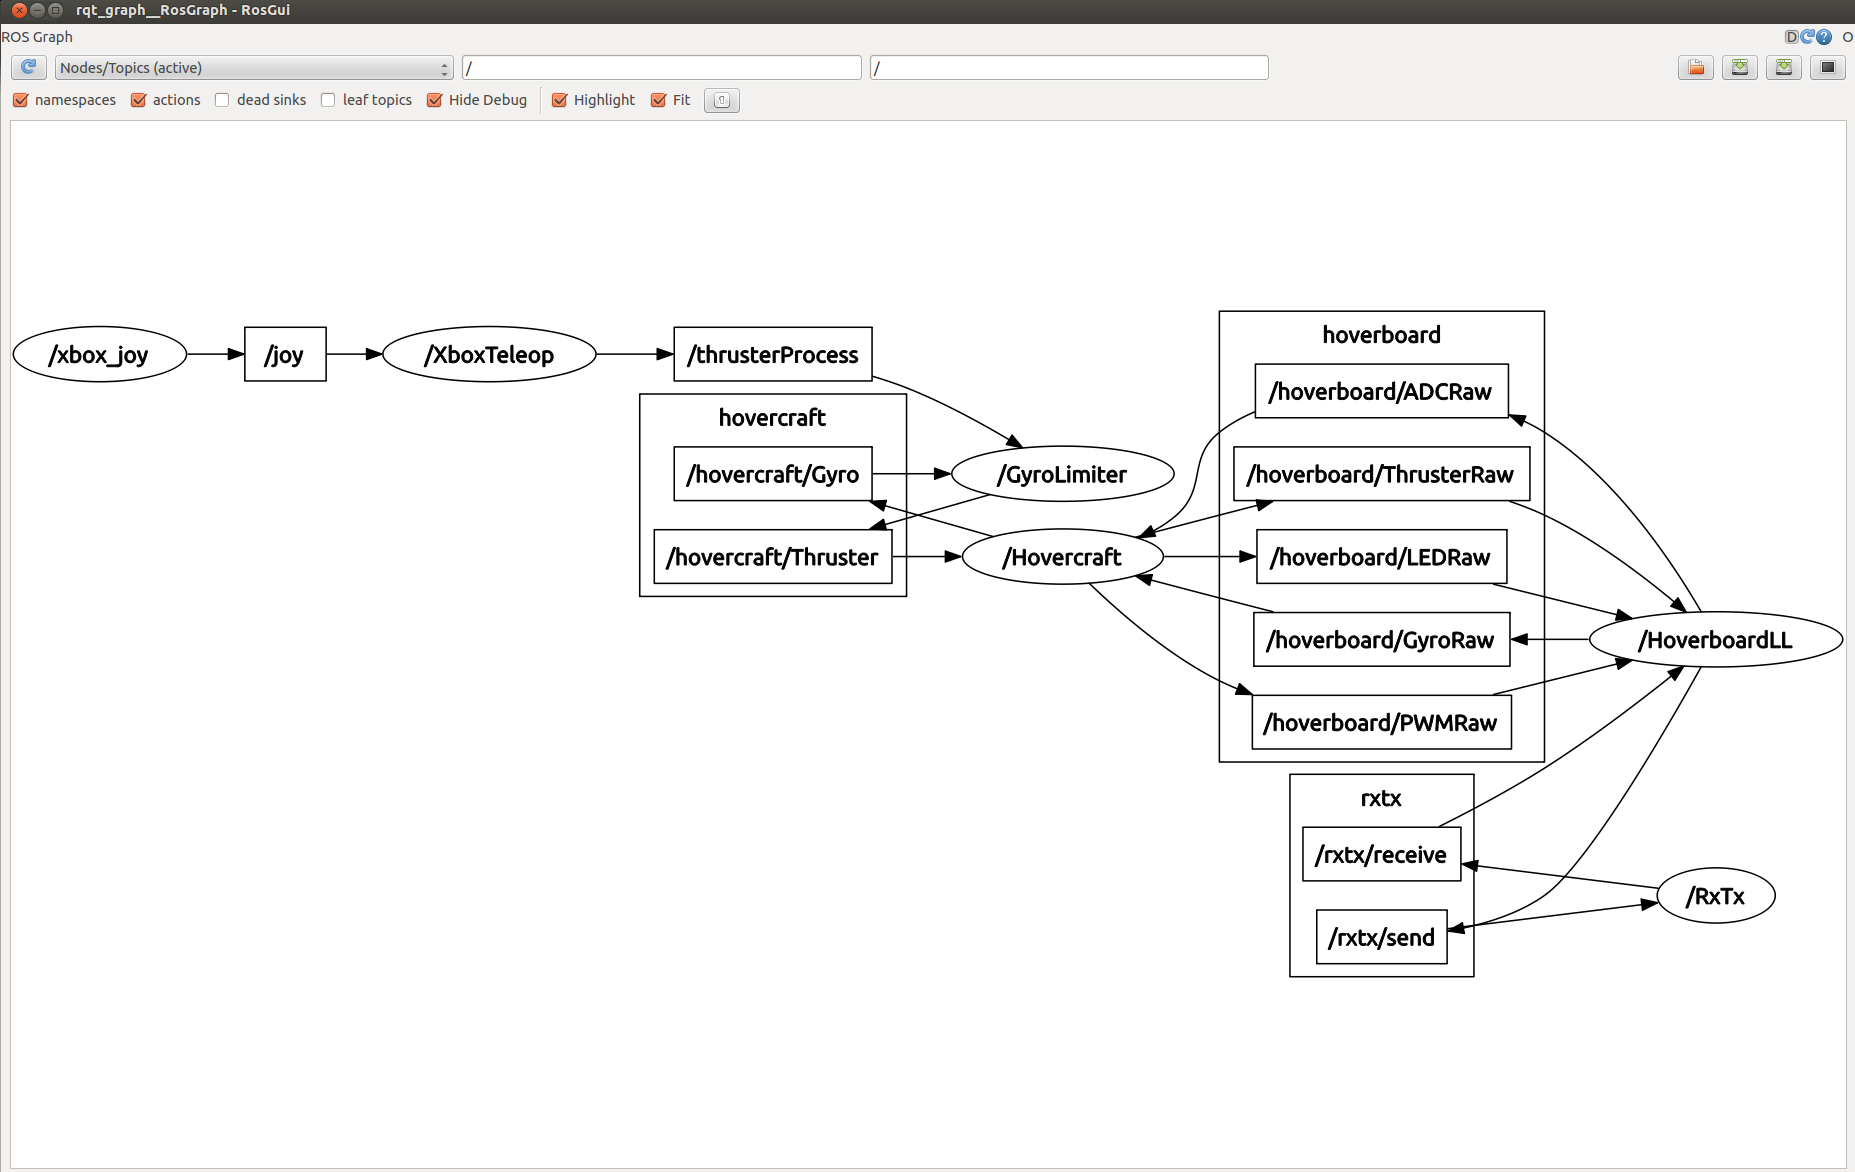
\includegraphics[width=1\textwidth]{images/rxgraph}
\caption{Structure of overall ROS system}
\label{rxgraph}
\end{figure}

Besides detecting the rotational rate of the hovercraft and controlling access to the thrusters, the hoverboard also provides some basic means of output in the form of LEDS.  These are controlled by sending messages on the topics  /hovercraft/LED and /hoverboard/LED.  The specific message types are hovercraft/LED and hoverboard/LEDRaw, respectively, though each is composed of the same basic information: a header and two 8 bit integers used to toggle the red and green light (1 for on, 2 for toggle, -1 to maintain the current value, and 0 for off).  Figure~\ref{rxgraph} shows the various nodes and messages used by the entire hovercraft, including the aforementioned LED messages.  

Often, it is extremely helpful (and sometimes necessary) to display the content of the messages being published on a topic in ROS.  For example, it may be necessary to view the rotational rate of the gyroscope in real time.  The command \emph{rostopic echo /hovercraft/Gyro} will do just that: any messages being sent on the topic /hovercraft/Gyro will be displayed on the standard output.  In this specific example, it's possible to view the header of the message, as well as the angle and rate of the gyroscope.  A similar command, \emph{rostopic hz /hovercraft/Gyro} will display the rate at which messages are being published on the given topic (in this case, the messages were published to /hovercraft/Gyro at a rate of 49Hz).  

In addition to simply viewing messages, it is possible to send messages to any given topic using the command \emph{rostopic pub}.  Using the LED messages above, it would be possible to toggle an LED on the hoverboard by issuing the command \emph{rostopic pub -1 /hovercraft/LED hovercraft/LED -- '\{led33\_red: 2\}}.  The specific format of the rostopic command can be divined by viewing the help message (\emph{rostopic pub --help}).  The parameters needed for the message (in this example, 
\{led33\_red: 2\}') can be determined using the command \emph{rosmsg show hovercraft/LED}.  

Sometimes, rosmsg will show two nearly identical messages (e.g., hovercraft/Gyro and hovercraft/GyroRaw).  These often measure the same information, but in different units or with different data types (pending on the implementation of the node).  For example, hovercraft/GyroRaw is bound between 0 and 360 and uses 16 bit signed integers to represent both the angle and the rate, but hovercraft/Gyro is uncapped (i.e., it can be any signed number), and each field is represented as a 64 bit float.  In this case, the units are the same as both messages measure the rate and angle in degrees and degrees per second, respectively.  This is easily determinable by viewing the message file defined in the node package.  

\begin{figure}
\centering
\subfigure{\label{maxposzoom}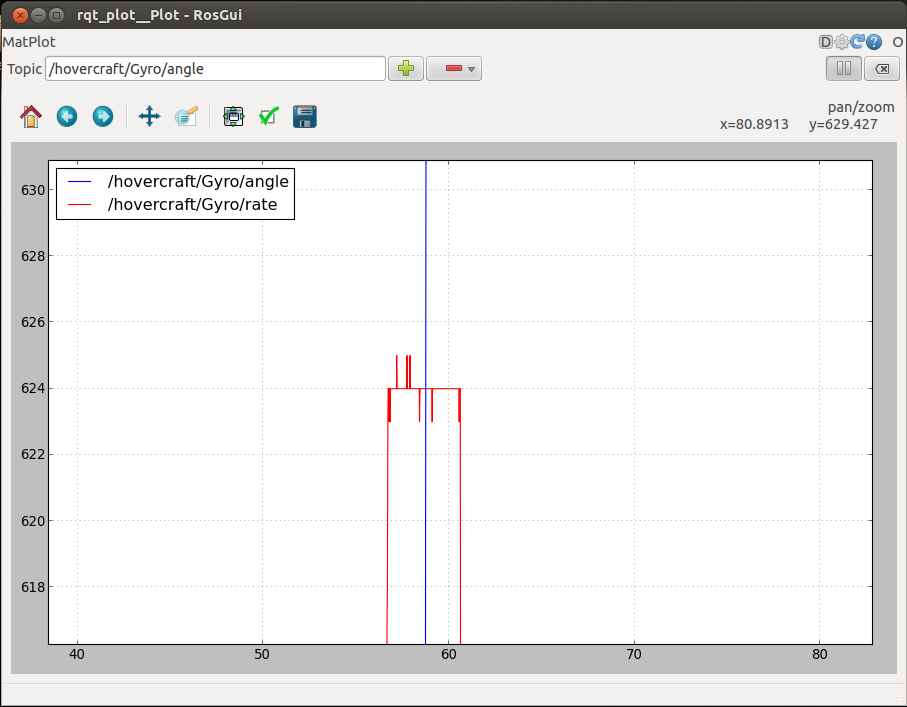
\includegraphics[width=.49\textwidth]{images/maxposratezoomed}}
\subfigure{\label{maxpos}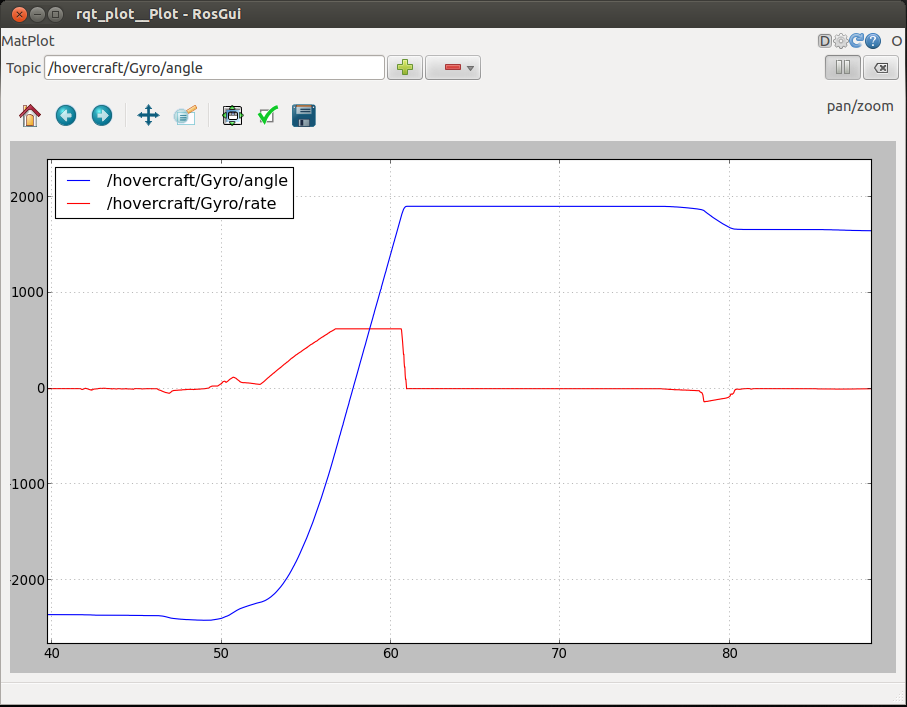
\includegraphics[width=.49\textwidth]{images/maxposrate}}
\caption{The maximum positive rotational rate of the hovercraft}
\label{maxposrate}
\end{figure}


\begin{figure}
\centering
\subfigure{\label{maxnegzoom}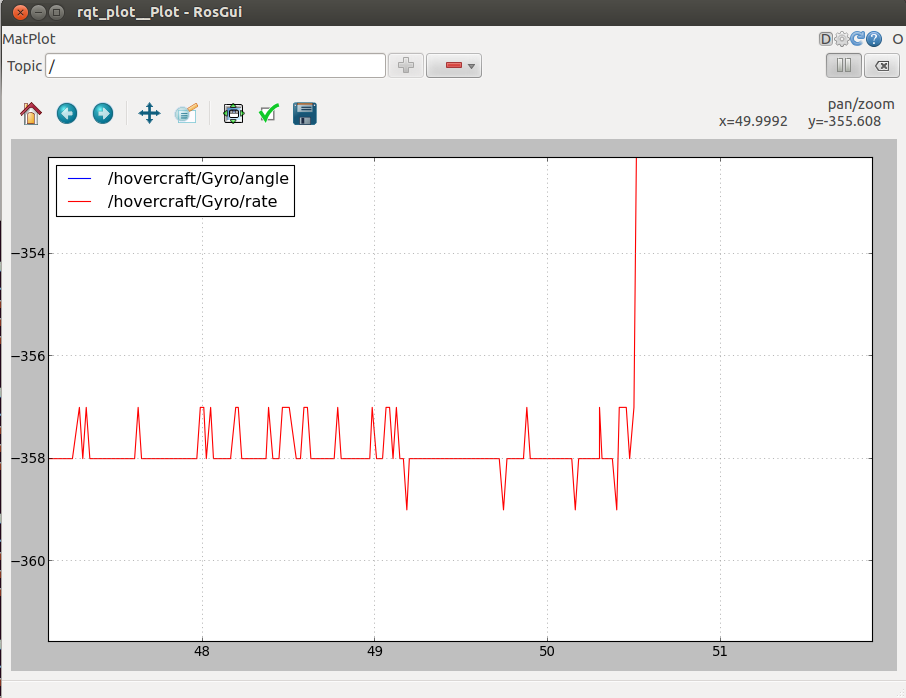
\includegraphics[width=.49\textwidth]{images/maxnegratezoomed}}
\subfigure{\label{maxneg}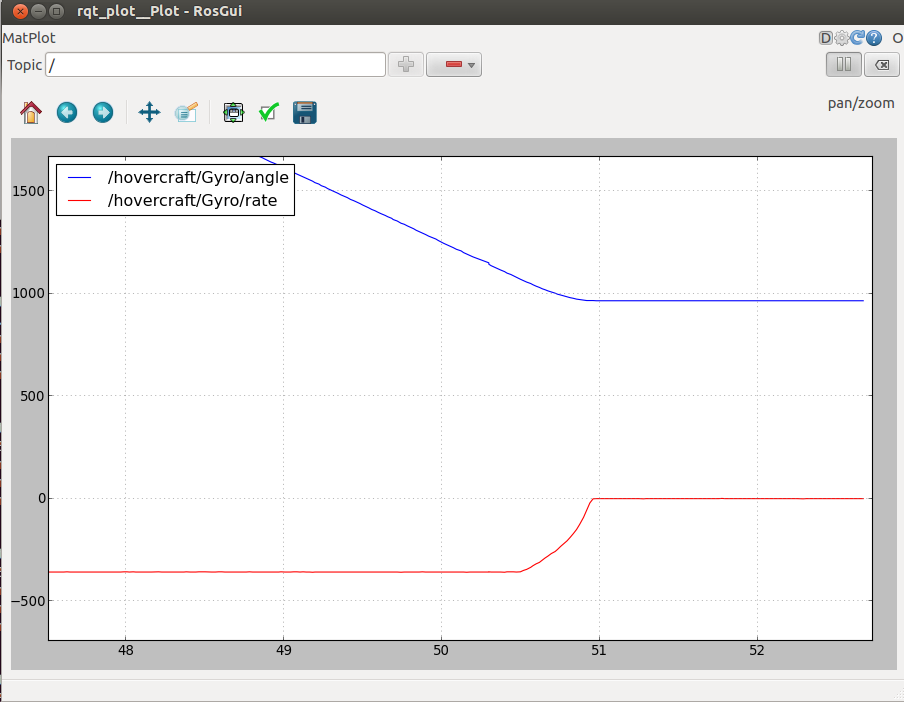
\includegraphics[width=.49\textwidth]{images/maxnegrate}}
\caption{The maximum negative rotational rate of the hovercraft}
\label{maxnegrate}
\end{figure}

Determining the specifics about the sensors can be done via simple experimentation in conjunction with rqt\_plot (a program that plots message data against time).  For example, to determine the maximum rotational rate that the gyroscope is capable of measuring, rqt\_plot was used to measure the /hovercraft/Gyro/angle and /hovercraft/Gyro/rate values while spinning the hovercraft at full thrust.  Figure~\ref{maxposrate} shows the maximum positive rate of spin in the counter clockwise direction (roughly 624$^\circ$/second).  The left plot shows a zoomed in version of the plot on the right.  Similarly, figure~\ref{maxnegrate} shows the maximum rotational rate in the clockwise direction (roughly 358$^\circ$/second).

%NOTE: It seems like the joy node only publishes 1 message with three members, but the handout leads me to believe otherwise
Aside from using preexisting nodes, ROS also enables users to write new nodes to add or modify the behavior of various components.  For example, publishing messages via rospub probably is not sufficient to enable fine tuned control of the hovercraft.  One solution is to use the existing joy node in ROS to publish commands from an Xbox controller using a new node (called XboxTeleop).  The joy node  itself
publishes three messages: a header, an array of floats corresponding to the joystick movements, and an array of integers corresponding to button presses. which will be used by the XboxTeleop node  

The axes message is mapped to the various Xbox inputs as follows:
\begin{itemize}
\item Index 0 and 1 correspond to the left joystick x and y axes (left/down correspond to negative values and vice versa).
\item Index 2 and 5 correspond to the left and right triggers (1 being the default position and -1 being fully depressed)
\item Index 3 and 4 correspond to the right joystick axes (identical to the left joystick axes)
\end{itemize}

The buttons have a similar mapping, with a value of 1 corresponding to pressed and 0 to unpressed:

\begin{table}[h]
    \begin{tabular}{|c|c|c|c|c|c|c|c|c|c|c|c|c|c|c|c|}
    \hline
    Button & a & b & x & y & L & R & Back & Start & Xbox & Left Joy & Right Joy & $\leftarrow$ & $\rightarrow$ & $\uparrow$ & $\downarrow$ \\\hline
    Index  & 0 & 1 & 2 & 3 & 4    & 5     & 6    & 7     & 8    & 9           & 10           & 11        & 12         & 13      & 14        \\\hline
    \end{tabular}
\end{table}

An effect of the joystick publishing at a high rate is that buttons will send multiple messages when pressed even fairly quickly.  This results in the (likely) unwanted effect of having the hovercraft's lift thruster rapidly turn on and off when the start button is pressed (assuming the start button is mapped to the lift thruster).  In order to prevent this from happening, the state of the start button was saved in the XboxTeleop node: if the button was depressed and a flag corresponding to the button being pressed was unset, the thruster was turned on and the flag was set.  The flag was unset when the start button was depressed, causing only the first press of the start button to turn on the lift thruster.  

%misnamed the picture...whoopsie.  Too lazy to fix.
Figure ~\ref{rxgraph} shows the rqt\_graph of the final system.  The XboxTeleop node was initially connected directly to the /hovercraft/Thruster message, allowing direct control of the thrusters via the Xbox controller.  However, an intermediary node was created (called GyroLimiter) that capped the maximum rotational rate of the hovercraft to the maximum rate detectable by the onboard gyroscope.  

\section*{Hovercraft Experiments}
To characterize the performance and limitations of the hovercraft, experiments were performed testing its thruster, rotational, and translational capabilities.  

 The minimum thrust power required to maintain lift was found to conserve power as well as preserve the integrity of the thruster.  This value was determined simply by starting at a low thruster value (specifically 0.2) and slowly turning the power on the thruster up until consistent lift was achieved.  While running the thruster at 0.2 was capable of providing lift, it had a tendency to sag due to unevenly distributed weight.  A lift power of 0.3 was found to be a reasonable compromise between lift power and conservation.  Giving the thruster more power would occasionally cause unwanted rotation ostensibly due to an uneven skirt.  This thruster force was enough to lift the hovercraft even with an additional .677 kilograms of mass onto of its base.  Additionally, with this extra mass, the hovercraft could still maintain lift and be moved after applying .55 newtons of force. 
 
The required force was calculated by measuring the displacement of a spring attached to the hovercraft, then determining the weight required to cause the same amount of displacement in the spring while being hung vertically.  The force could then be determined by using the equation $f=kx$, where $k$ is a spring constant and $x$ is the displacement of the spring. Because $k$ was unknown for the spring that was used to conduct the experiment, it was simply ignored, likely causing a small amount of error in the calculated force required to move the hovercraft with additional weight.  The same experiment was repeated for the hovercraft with no additional weight.  However, the amount of displacement of the spring was immeasurable using the conventional and readily available methods.  This means a very small (near negligible) amount of force was required to move the hovercraft on its own.

In addition to conserving the main lift thruster power, thrusters 4 and 5 (i.e., the rotational thrusters) were capped at the maximum rotational rate detectable by the onboard gyroscope.  This rate (seen in figures~\ref{maxposrate} and~\ref{maxnegrate}) ranged from -358$^\circ$/second to 624$^\circ$/sec.  To limit the rate, an additional node was created called GyroLimiter, which was subscribed to both /hovercraft/Gyro and /thrusterProcess (as seen in figure~\ref{rxgraph}).  GyroLimiter acted as an intermediary node between the XboxTeleop node and the thrusters themselves: If the XboxTeleop node sent a rotational command to the GyroLimiter and the gyroscope was reporting the maximum rotational rate (either positive or negative), the corresponding rotational thruster was shut off and any additional input sent to that thruster was ignored for a brief period (1 second) to prevent rapid oscillations.  
\begin{figure}
  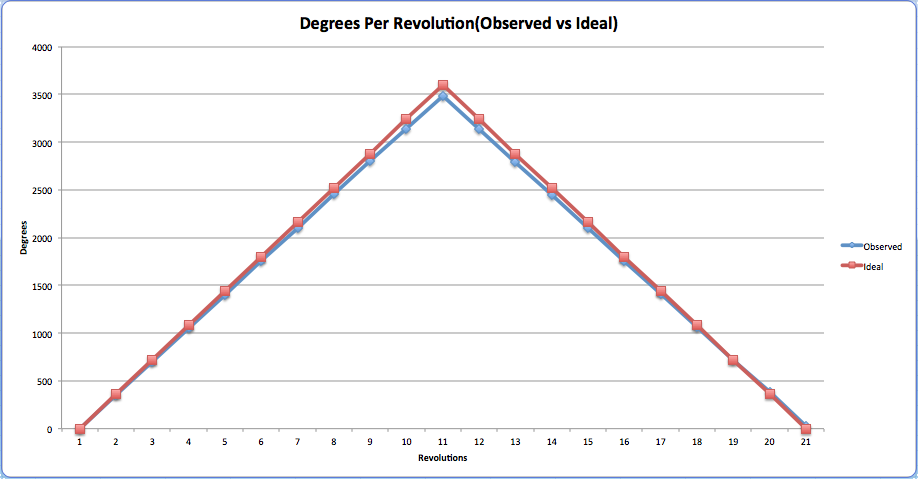
\includegraphics[width=.85\textwidth]{images/revs}
  \caption{The ideal vs actual degrees detected by the gyroscope after 10 revolutions}
  \label{revs}
\end{figure}

\begin{table}
 \caption{Degrees per Revolution}
 \begin{tabular}{| r | c | c | c | c | c | c | c | c | c|c|c|}
    \hline
    Observed & 0 &  350 & 701 & 1050 & 1403 & 1753 & 2105 & 2455 & 2802 & 3140&3480\\\hline
    Ideal & 0 & 360 & 720 & 1080 & 1440 & 1800 & 2160 & 2520 & 2880 & 3240 &3600\\\hline\hline
    Observed  & 3137 & 2795 & 2447 & 2102 & 1756 & 1411 & 1068 & 723 & 379 & 33&\\\hline
    Ideal & 3240 & 2880 & 2520 & 2160 & 1800 & 1440 & 1080 & 720 & 360 & 0 & \\\hline
    \end{tabular}
    \label{revtable}
\end{table}

The rotational rate range is not the only limitation of the gyroscope.  The gyroscope suffers from a loss of accuracy over several revolutions.  To determine how much the gyroscope deviated from the actual amount of rotation, the hovercraft was rotated a full 360$^\circ$ in one direction, ten times in a row.  At each revolution, the gyroscope's sensor was read and compared with the actual number of degrees the hovercraft had been rotated (in this case, the actual number was always in multiples of 360).  Table~\ref{revtable} shows the exact values obtained from this experiment, and figure~\ref{revs} shows a plot of the same data.  On average, the gyroscope loses roughly 10$^\circ$ per rotation.  Additionally, when the hovercraft was rotated in the opposite direction the same number of times, the angle should have (ideally) read at 0$^\circ$.  However, the observed reading was 33$^\circ$, meaning there is a different loss of accuracy pending on the direction of rotation.

Configuring and characterizing the thrusters to effect translational movement was significantly more time consuming than examining the gyroscope or lift thruster.   Figure~\ref{hovercraft} shows the hovercraft with the forward position towards the top of the image.  To move forward, left, or right, two thrusters were required to provide thrust at the same time.  However, left and right translation required the two thrusters to operate at different levels due to their orientation.  Forward translation required thrusters 2 and 3 to operate in equal proportion to one another.  Left translation required thrusters 1 and 3, with thruster 3 supplying 3 times the amount of thrust.  Similarly, right translation required thrusters 1 and 2 to fire, but with thruster 2 providing 3 times the amount of thrust.  Backward translation required only thruster 1 to fire.

To enable finer control over the translational movements of the hovercraft, an equation was derived using the known angles between thrusters.  Specifically, if the desired angle to move in is $\theta$ and all thrusters provide the same thrust at the same power level, then $\theta = \arctan(\frac{yAxis}{xAxis}) * \frac{180}{\pi} + 180)$ (the addition of 180 normalizes the angle to [0,360]).  The power needed for each thruster was then determined by finding the hypotenuse of the triangle formed by x and y axes of the joystick.  This enabled the hovercraft to simultaneously 

To test the translational abilities of the hovercraft,  the hovercraft was driven over tape on the floor that formed something resembling a star pattern with edges at roughly 45$^circ$ angles.  The goal was to translate along one edge of the pattern, then back, and continue along different edges until each translational direction had been tested.  Overall, the hovercraft performed admirably: it was capable of moving at the desired angle, but typically deviated from the path when stopping due to a slight rotation (likely due to weight balance issues) and inertia.  

To remedy inertial effect the lift power was decreased to increase the friction of the hovercraft.  To curb the rotational effects somewhat, the thrusters were manually calibrated to attempt to decouple the translation and rotation.  Adopting a different equation (perhaps a vector based algorithm) or altering the layout of the thrusters on the hovercraft might produce better translational capabilities (or by adding an additional thruster to the hovercraft, mitigating the need to fire two thrusters simultaneously).


\section*{Conclusion}
Designing, assembling, and programming a hovercraft turned out to be a more arduous and time consuming task than initially thought.  The task involved a fair amount of handiness, programming skills, and mathematical knowledge to complete.  To streamline the entire process, two groups were formed: Baoliang Zhao and Lina Yu each spent 12 hours building the hardware, running the translation and force test experiments, and manually calibrating the thrusters.  Kevin Chiang and Tony Schneider spent roughly the same amount of time programming, testing, and getting the translational controls to work.  One of the most trying and difficult pieces of functionality to design was the translation algorithm, with a close second being the manual calibration of the thrusters. However, the hardest part of design may have been finally settling on a name: Dopey (though, Puck, Sunny, Halo, and Drifter were all close runner-ups).
\end{document}